%
% Chapter 3 - Results
%
\chapter{Results}

This chapter highlights the final results of the project,
including every decision made by the group and tangible accomplishments for each developed module.\\

\newpage
\section{Relational database}

Which database should be used is one of the first and most
crucial steps after determining functional requirements 
as it establishes the data's model and how the communication
with the server will be made, meaning that a wrong choice
would cause major restructures.\\

Before adopting a specific database, one should first
consider between a relational model and a No-SQL model. 
Given the complex hierarchy between data entities,
tutor's considerations and the need for a model capable of 
providing quick results when querying around a geolocation, 
a relational model was chosen.

\subsection{Used tecnologies}

When the project was in a planning phase, the group decided that a relational database was the most suitable option for this project
instead of a No-SQL database, because of the project's structure - there are many hierarchies between entities, which invalidated the
no-SQL option.\\

Out of all researched relational databases, 
PostgreSQL was chosen as it supports the PostGIS\cite{postGIS} plugin, and 
is supported by Heroku - allowing to 
deploy the application in later stages of development.\\

\subsection{Conceptual model}
As a result of multiples redesigns, here is the database's conceptual model.

\begin{figure}[H]    
    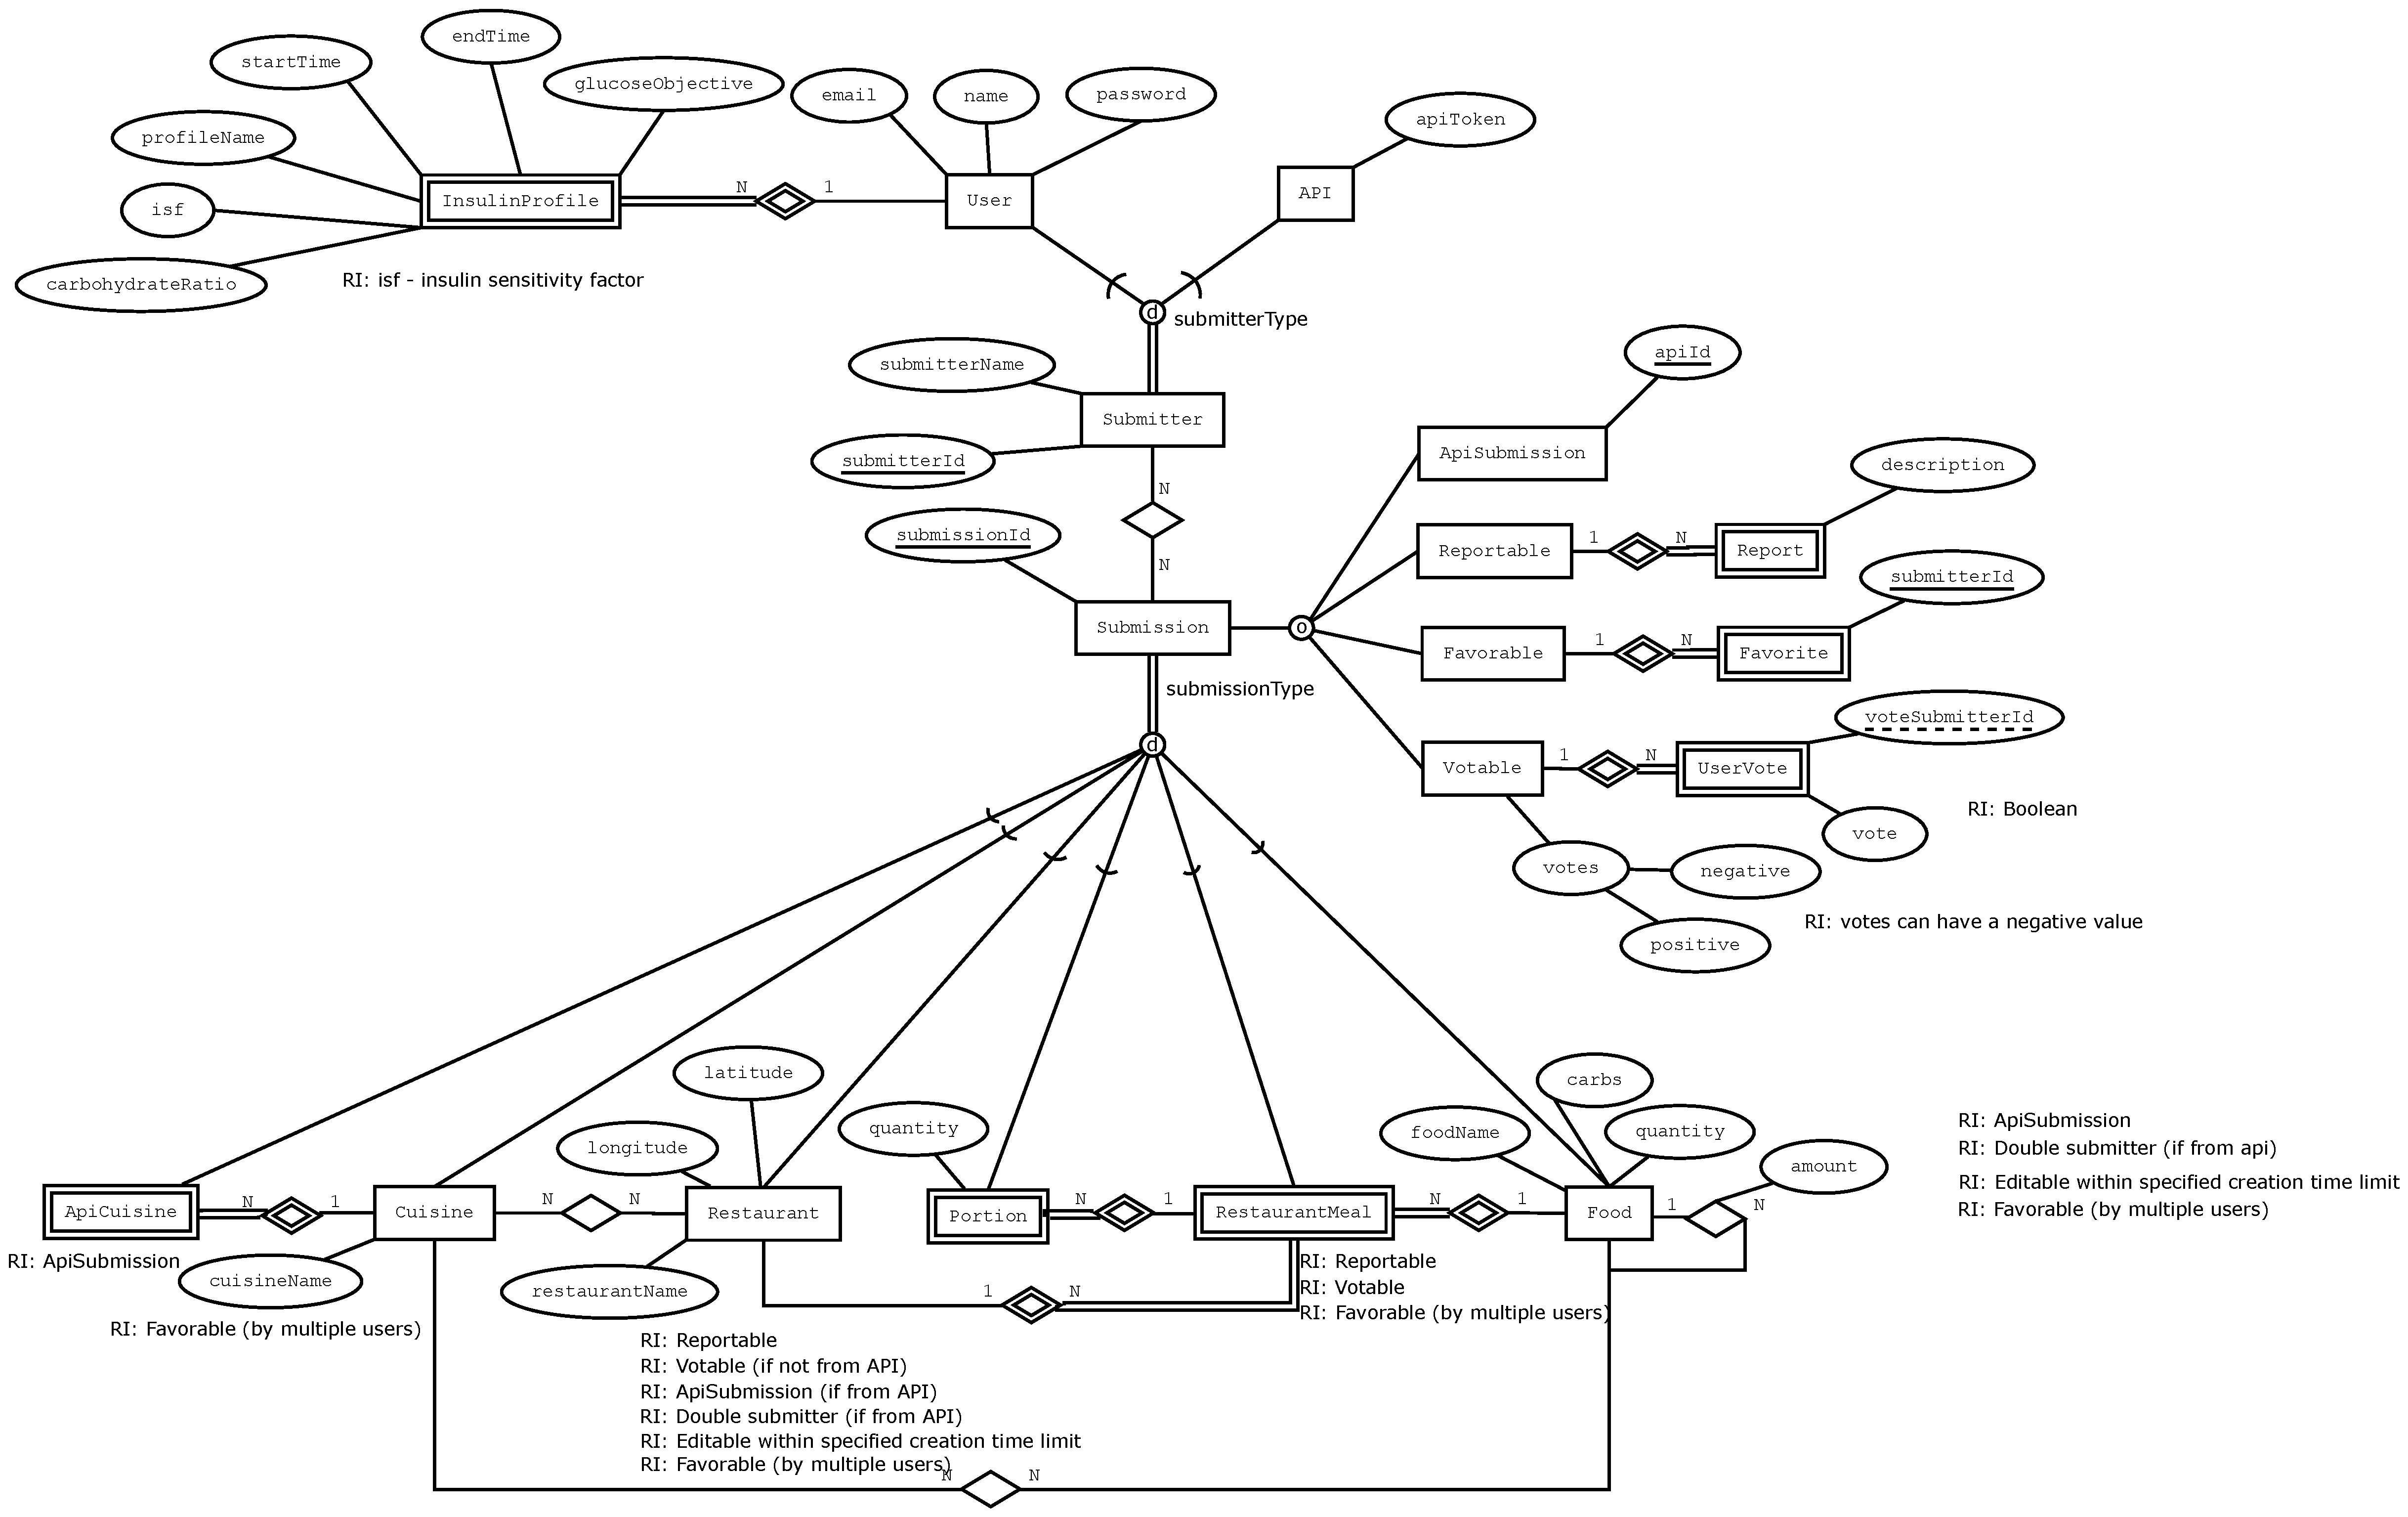
\includegraphics[scale=0.2]{_figures/Nutr.io_Database_Diagram.eps}
    \caption{Database conceptual model}
\end{figure}

The database's relational model is present inside this report's appendix [\nameref{app:relational_model}].\\

In the relational model there are tables which are not specified in the conceptual model.
These are a product from associations between entities which will simplify queries' complexity.\\

Now the submission can fall into 4 categories: ApiSubmission, Reportable, Favorable and Votable, in order to disguish between submissions that
are from the user or from APIs and to separate which ones can be reportable, favorable and votable by the user.\\

The cuisine entity has now an associated entity called ApiCuisine, to save cuisine information provided by the Here API.\\

Meals and ingredients were now condensed into one entity called food - now each meal can have meals inside it that can also be considered
ingredients in other contexts.\\

Therefore each meal possesses nutritional information, which is essential to the user especially to the insulin calculations. That information is composed by
'carbs' - meal's carbohydrates; and quantity - meal's quantity.\\

\section{HTTP server}

\subsection{Used tecnologies}

\subsubsection{Kotlin}

The group chose to use Kotlin\cite{kotlin} for the HTTP server developed as it is a language that is being more adopted and used nowadays and because it is totally 
interoperable with Java\cite{java}.\\

It was also the language used during PDM, which is an optional course for Android application development inside the LEIC programme, 
making this a language the group felt confortable with.\\

\subsubsection{Spring MVC}

At the beginning of the project the group decided to use Spring MVC\cite{springmvc} rather than Ktor\cite{ktor}, as the first one is taught in DAW, which is an optional course
for Web applications development inside the LEIC programme. As Spring MVC has a better coverage inside the LEIC programme, the group considered 
it a more solid choice.\\

\subsubsection{Used dependencies}

Here are all the dependencies injected inside HTTP server gradle settings file.\\

\begin{itemize}
    \item \textbf{Kotlin base dependencies} - kotlin-reflect and kotlin-stdlib-jdk8;
    \item \textbf{Spring base dependencies} - spring-boot-starter and starter-web;
    \item \textbf{Mockito} - for tests with mocks;
    \item \textbf{Jackson} - for JSON serialization and deserialization;
    \item \textbf{JDBI} - the driver/interface for connecting with the relational database;
    \item \textbf{Spring Security} - for authentication and authorization proposes.
\end{itemize}

\subsection{Code structure}

\textbf{TODO - eng. Félix says: "Needs more information about the backend organization, such as: intermediaries, controllers, services, database access method, external dependencies used"}

\begin{figure}[H]
    \begin{center}
        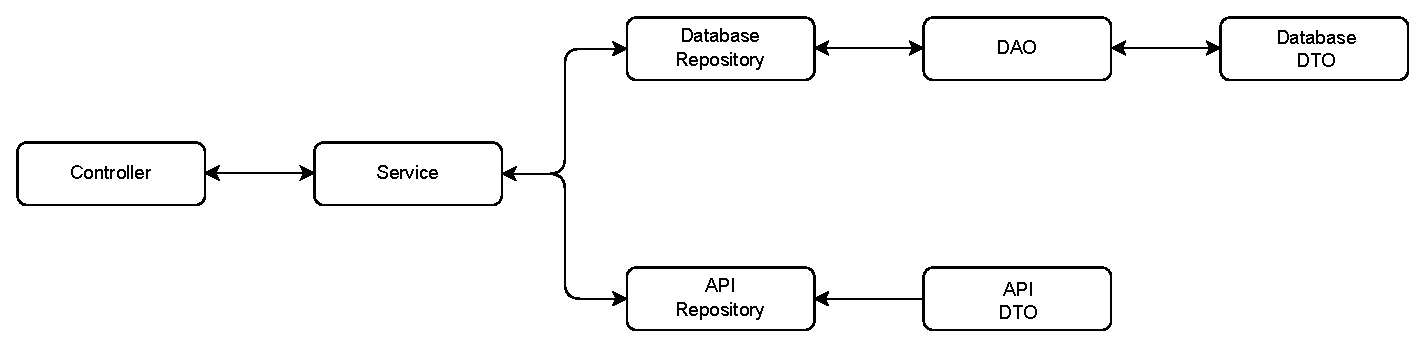
\includegraphics[scale=0.7]{_figures/server-classes.eps}
        \caption{Server's classes structure}
    \end{center}
\end{figure}

\subsection{JDBI}

After some discussion of which driver should be used to allow communication between the server and database, the group decided that the JDBI\cite{jdbi} was the best
option as it is a library built on JDBC\cite{jdbc}.\\

The library also exposes two different API's styles: a fluent/imperative style and a declarative style (used during development), as shown below.

\begin{figure}[H]
    \begin{center}
        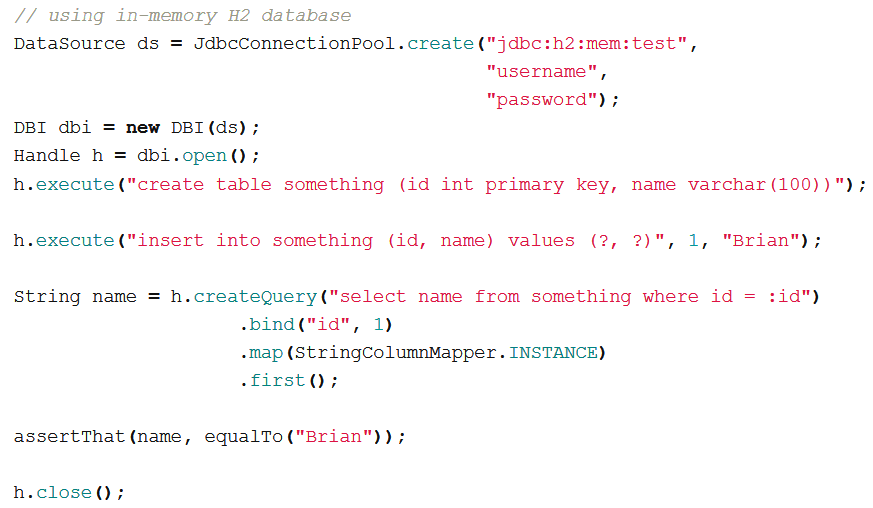
\includegraphics[scale=0.5]{_figures/fluentApiJdbi.png}
        \caption{JDBI using an imperative API style}
    \end{center}
\end{figure}

\begin{figure}[H]
    \begin{center}
        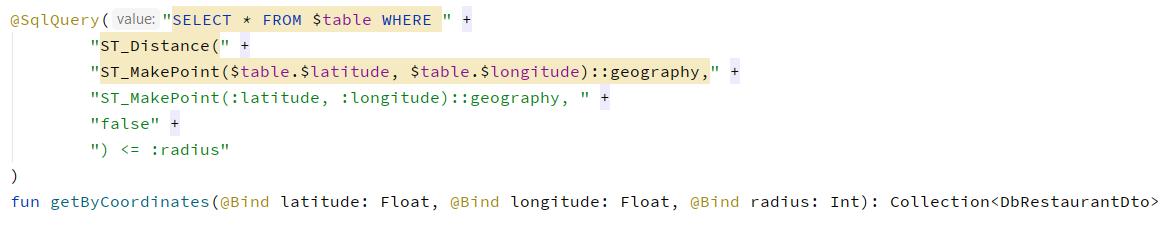
\includegraphics[scale=0.5]{_figures/sqlObjectJdbi.png}
        \caption{JDBI using a declarative API style (example from HTTP server)}
    \end{center}
\end{figure}

The group chose to use a declarative style due to its convenience and code simplicity
over the imperative one. It was also the more adequate style to the project's structure. 

\subsection{Spring Security}

\subsubsection{JSON Web Tokens}

As each client needs to have authentication to provide the user a way to create an account and allow submissions and data synchronization,
the group had to discuss about the platform's security and the safest ways to do that.\\

It was concluded that the use of \textbf{JSON Web Tokens}\cite{jwt} was the best option, because of the nature of the clients, more specifically the fact that
the mobile application is completely \textbf{stateless}.\\

Another advantage is the fact that these tokens have an expiration time, which means that after a certain amount of time they are no longer valid.
In case of security breach, this feature becomes useful, because if the attacker does not have a way to generate valid tokens neither does not know the user password and steals 
a valid token, this will only be used by a short period of time (10h), easing the amount of damage that an intruder can make and confining it to 
only one user inside the platform.\\

The picture below represents a very generic and simplified workflow of the JSON Web Token. 

\begin{figure}[H]
    \begin{center}
        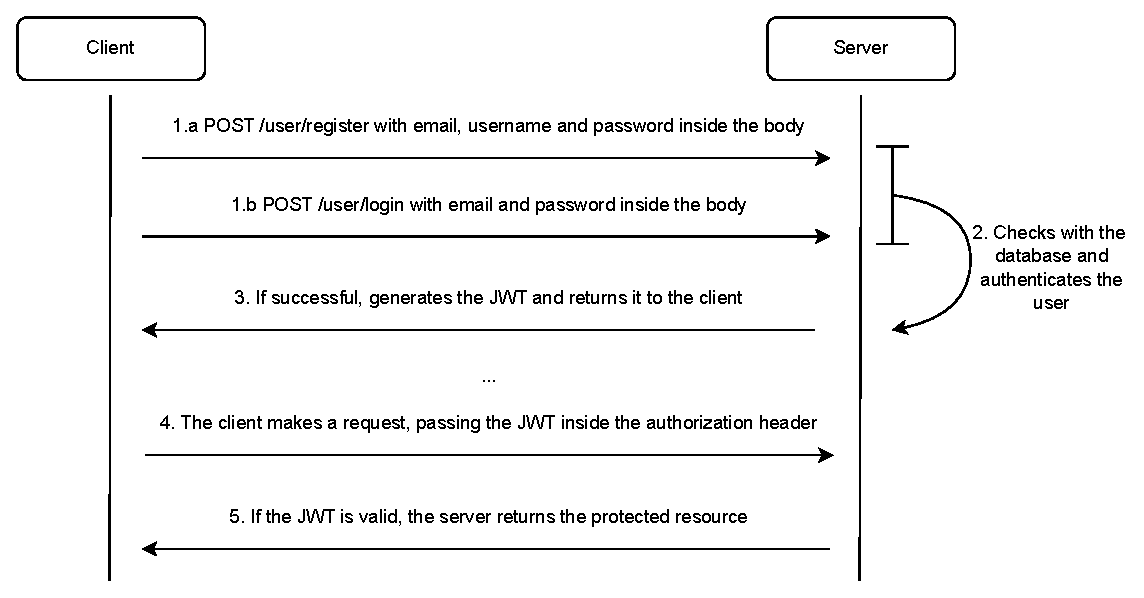
\includegraphics[scale=0.9]{_figures/JWT-simple-diagram.eps}
        \caption{The JWT workflow}
    \end{center}
\end{figure}

\subsubsection{Implementation}

To implement the shown workflow inside the HTTP server, as the group is implementing it with Spring, the more obvious choice was to use \textbf{Spring Security}\cite{springsecurity}.\\

Spring Security is a customizable authentication and access-control framework.\\

The picture below shows how the server handles a user login usin this framework.\\

\begin{figure}[H]
    \begin{center}
        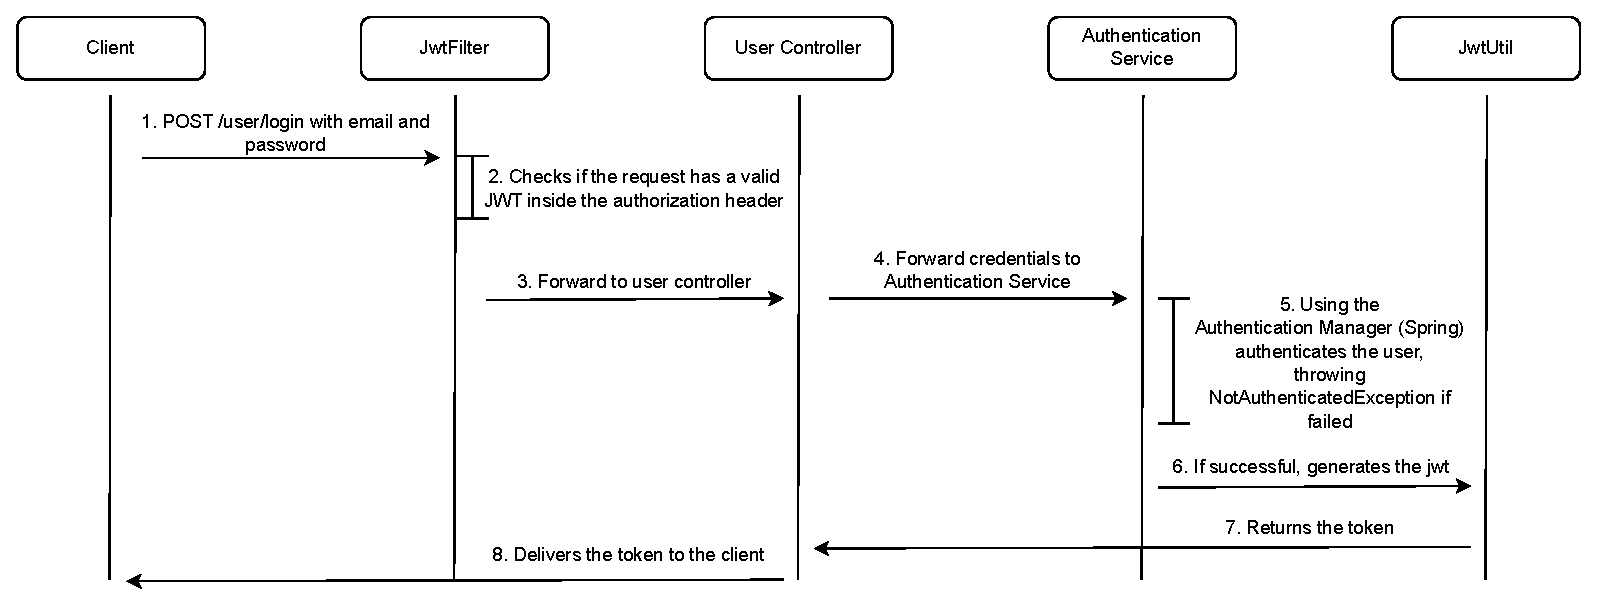
\includegraphics[scale=0.65]{_figures/Spring-jwt-diagram.eps}
        \caption{A Spring security workflow example with the POST /user/login}
    \end{center}
\end{figure}

After the previously mentioned dependencies are installed, the WebSecurityConfig is the first class to be constructed. Here are specified, via antMatchers, which
endpoints do not need authentication, acting like a whitelist, so every endpoint that is not specified via antMatchers needs authentication, and will return code 401
Unauthorized if the JWT is invalid or absent. The JWT filter is also started up inside this class.\\

The Jwtfilter class, as the name says, filters each request, checking the authentication header and extracting the jwt from the Bearer
verifying if it is valid. This class extends the OncePerRequestFilter() which garantees a single execution of this filter every request.\\

The Authentication service class calls the Spring Authentication Manager and authenticates the user, it provides methods which call the JwtUtil
to retrieve the email from the token or encode the password when registering.\\

The password encoding always happens when the user registers for the first time: the server hashes the password using \textbf{BCrypt} before inserting the new
user into the database.\\

BCrypt\cite{bcrypt} is a password-hashing function based on the Blowfish\cite{blowfish} cipher. The group found this function very convenient for these reasons:
\begin{itemize}
    \item Already pre salts the passwords, preventing rainbow table attacks\cite{rainbowtable};
    \item Makes bruteforce attacks inviable: the iteration count can be increased to make it even slower to crack.
    This cipher makes even GPU-powered bruteforce attacks impracticable due to this feature.
\end{itemize}

The JwtUtil is the core class which validates, generates and adds claims to the tokens.\\

\section{Geolocation}

Given how all clients rely on obtaining nearby restaurants, there was a need to implement a geolocation function in the project's design.\\

Initial research showcased two possible solutions: Haversine\cite{haversine} distances and cartesian distances, where the latter returns a highly imprecise distances.
As such, Haversine was selected.\\

The next step was to choose which system filters nearby restaurants: database or HTTP server. After some discussion, the group decided that database was the best
option for two reasons: 
\begin{itemize}
    \item Given the large amount of existing restaurants, sending such data from the database to the HTTP server so that it could filter it would occupy too much memory;
    \item PostgreSQL already supplies extensions that add support for location queries, namely PostGIS.
\end{itemize}

\section{Android application}

\subsection{Used tecnologies}

\subsubsection{Kotlin}

The group chose to use Kotlin for the mobile application development, as it is now the official programming language for Android development,
according to Google.\\

It is also the language taught during the optinal course - mobile devices programming (PDM)\\

\subsubsection{External dependencies}

Here are the dependencies that were included in the mobile application which gave more functionalities to it.

\begin{itemize}
    \item \textbf{Volley} - an HTTP library for Android networking;
    \item \textbf{Jackson} - JSON serialization, deserialization and handling;
    \item \textbf{Room} - A framework to store data locally;
    \item \textbf{MapBox} - A framework to provide maps and geolocation tools;
    \item \textbf{MPAndroidChart} - provides custom graphs inside the application;
    \item \textbf{Glide} - a framework for image loading;
    \item \textbf{Androidx crypto} - a new crypto library made by Google, used to encrypt User credentials.
\end{itemize}

\subsection{Code structure}

\subsubsection{Drawing pattern}

The mobile application code structure follows the \textbf{repository pattern}, which is a code architecture recommended by the \textbf{Android Jetpack}\cite{jetpack} for this type of applications.\\

\begin{figure}[H]
    \begin{center}
        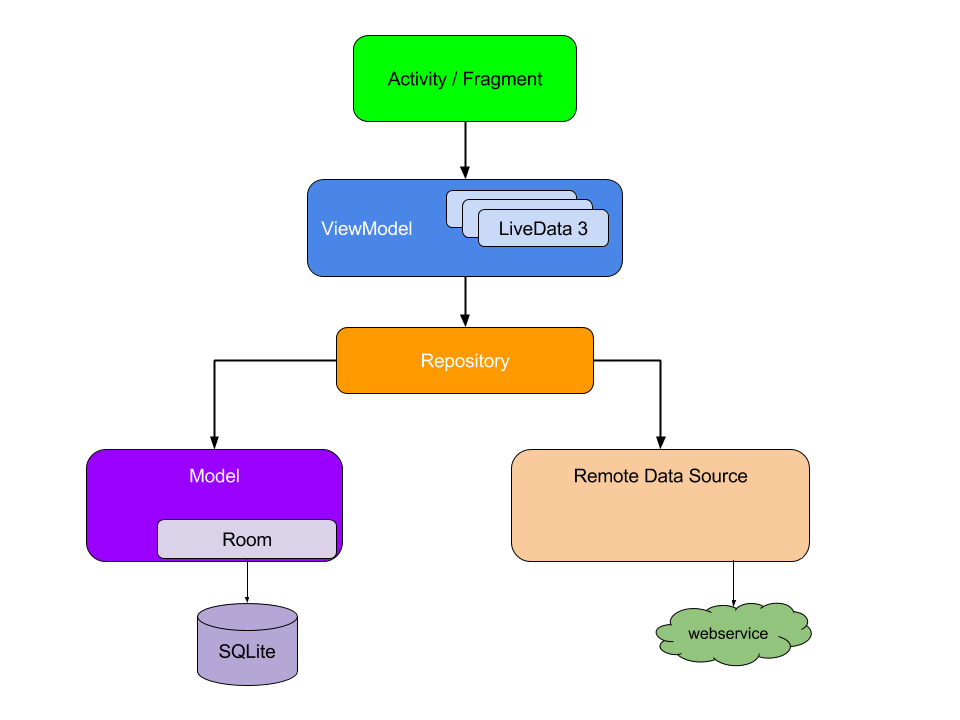
\includegraphics[scale=0.5]{_figures/repository_pattern2.png}
        \caption{The repository pattern diagram}
    \end{center}
\end{figure}

Above there is the pattern's diagram provided by the Android Jetpack.\\

The idea behind this architecture is that each Activity or fragment has its own ViewModel and each one calls the needed functions present inside the repository.
The repository is a layer that manages where the information should be retrieved from.\\

The 'DTO to model' mapping also occurs inside the repository, following the rule where ViewModels should only manipulate models and the layers below should only use DTOs.\\

By following this pattern, the code becomes segmented and organized, allowing a good comprehension and code maintainability.\\

\subsubsection{Fragments}

The group chose to use fragments\cite{fragment} for each application view instead of activities. Although a fragment has a more complex lifecycle than the activity and depends on it
to exist, they are far more lightweight to instanciate than an activity and thus they provide more performance to the application.\\ 

It is also the recommended Android widget to use when designing an application with a side drawer.

\subsection{Local data storing}

As mentioned in the dependencies, the mobile application utilizes Room to store data locally. This is convenient
for multiple reasons: 
\begin{itemize}
    \item To allow using the application in offline situations;
    \item To save data in order to avoid unnecessary requests to the server;
    \item To help data synchronization, that will be detailed later in this section.
\end{itemize}

\subsection{User authentication and authorization}

The user has the ability to register and login in the mobile application. Besides being the server responsable for these functions, the mobile application has also some intervention
here, because after a successful login or register, the HTTP server will return a jwt (JSON Web Token) that will authenticate and authorize the user in future requests.\\

This token will be stored in the Android Shared Preferences\cite{sharedpreferences} and it will also to be renewed periodically due to its 10h expiration time. The user credentials will also be saved
inside the mobile device to allow automatic logins to renew the user's JSON Web Token and avoid its expiration.\\

\subsubsection{Problem: The content inside the shared preferences is written in plaintext. Is it safe to store user credentials inside the shared preferences?}

Although the Android Shared Preferences being a safe place to store application information, this fact is not completely true:
a normal device can not access these preferences and it should be a safe place to store user credentials, however rooted devices can easily
access the shared preferences file and retrieve plaintext from it, which would compromise the user security.\\

\subsubsection{Resolution: Androidx Crypto}

The Androidx crypto\cite{crypto} was used to solve this issue. This library is used to encrypt the user credentials before writing them inside the mobile device.\\

These new Google library takes advantage of the Android KeyStore\cite{keystore} system, which encrypts information using a hardware-level encryption, making the
encryption even harder to break. The information is encrypted using a symmetric cipher algorithm (AES-256), the key used to sign and encrypt information
is hardware-generated and it is managed by the application itself, so the key's retrieval from an 'encrypted' shared preferences is equal to the 'normal'
shared preferences.\\

The group also discussed if the credentials should be saved inside the device or if only the database should possess them.
If that approach was taken, the user had to login each time it was needed to read or write a protected resource.\\

As this platform is not, for example, a bank application that needs top protection. The group found this level of protection
unnecessary for the application and inconvenient for the user and decided that only the essential protection should be provided - 
user credentials encryption to avoid information leaks from rooted devices.

\subsection{Data synchronization}

Background data synchronization will happen after a successful login or register. The only user data that will be synchronized are:
\begin{itemize}
    \item Insulin profiles;
    \item Custom meals made by the user;
    \item Favorites.
\end{itemize}

When logged in, the data can be synchronized in two ways:
\begin{itemize}
    \item the user forces the synchronization by swiping down on a list;
    \item The Android WorkManager will make sure that the data is synchronized at least once a 
    day when the phone is inactive and connected to the internet.    
\end{itemize}

\subsection{Android version compatibility}

In order to garantee a global support by most of the Android devices nowadays, the mobile application is supported since \textbf{Android 7} (API level 24)
up to \textbf{Android 10} (API level 29).

\subsection{Functionalities}

Here will be displayed pictures of the mobile application and its functionalities, explaining each one.\\

\textbf{This section will be completed in the final release, once every UI aspect is resolved}

\section{Web browser application}

\subsection{Used tecnologies}

\subsubsection{React framework}

The group chose to build the website with JavaScript \cite{javascript} using the React framework \cite{react} , as it was the framework lectured in the Web applications
development course and has innumerous advantages to other frameworks, such as Node.JS.

\subsection{Code structure}

\subsubsection{Single-page application}

As website design pattern, the group chose to conceive a single-page application. This pattern was chosen for a 
variety of reasons, being the main one a better performance comparing to a traditional multi-page application.\\

\subsubsection{Routing}

\textbf{Under development}

\subsection{Functionalities}

\textbf{Under development}
